\subsection{Hypothesentests - Allgemein}

\label{sec:hypothesengrundlagen}

\begin{description}
    \item[Nullhypothese] ($H_0$): 
        Wird als "Standardannahme" betrachtet, die gilt, solange keine
        ausreichende Beweisefür das Gegenteil vorliegen.

    \item[Alternativhypothese] ($H_1$): 
        Beschreibt, was man beweisen möchte. 

    \item[Fehler 1. Art] ($\alpha$): 
        Zu Optimistisch. \\
        Tritt auf wenn die Nullhypothese ($H_0$)
        abgelehnt wird, obwohl sie \textbf{wahr} ist.
        Die Wahrscheinlichkeit eines Fehlers 1. Art entspricht dem festgelegten
        Signifikanzniveau.

    \item[Fehler 2. Art] ($\beta$): 
        Zu Vorsichtig. \\
        Tritt auf wenn die Nullhypothese ($H_0$)
        \textbf{nicht} abgelehnt wird, obwohl sie wahr ist.

    \item[Signifikanzniveau] ($\alpha$): 
        Wahrscheinlichkeit, die einen
        Fehler 1. Art zulässt (in Prozent, z.B.: $5\%$).

\end{description}

\vspace{1cm}


\begin{center}
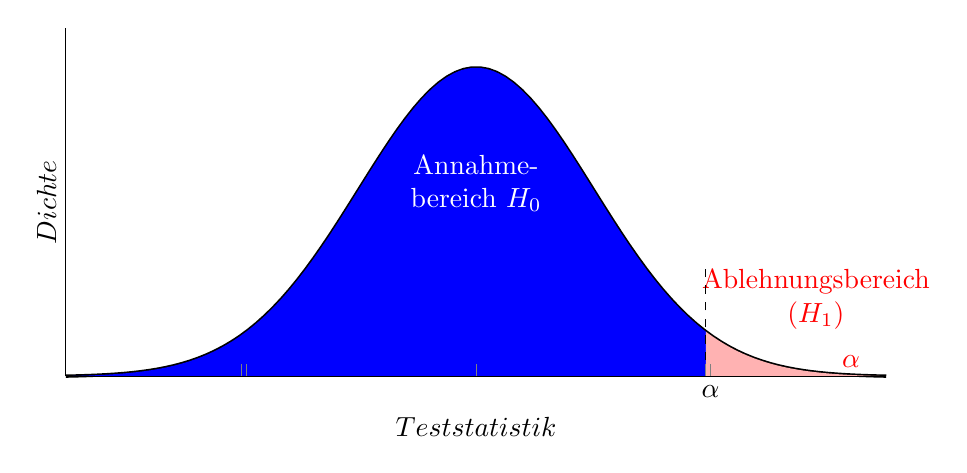
\begin{tikzpicture}
    \begin{axis}[
        no markers,
        samples=100,
        domain=-3.5:3.5,
        ymax=0.45,
        axis lines*=left,
        xlabel={\(\text{Teststatistik}\)},
        ylabel={\(\text{Dichte}\)},
        xtick={-2,-1.96,0,1.96,2},
        xticklabels={,,,,\({\alpha}\)},
        ytick=\empty,
        enlargelimits=false,
        clip=false,
        axis on top,
        height=6cm, width=12cm
    ]
    \addplot [very thick, black] {exp(-x^2/2)/sqrt(2*pi)};

    \addplot [
        draw=none,
        fill=blue,
        domain=-3.5:1.96
    ] {exp(-x^2/2)/sqrt(2*pi)} \closedcycle;

    \addplot [
        draw=none,
        fill=red!30,
        domain=1.96:3.5
    ] {exp(-x^2/2)/sqrt(2*pi)} \closedcycle;

    \node[align=center, white] at (axis cs:0,0.25) {Annahme-\\bereich \( H_0 \)};
    \node[align=center, red] at (axis cs:2.9,0.1) {Ablehnungsbereich\\ (\( H_1 \))};

    \draw[dashed] (axis cs:1.96,0) -- (axis cs:1.96,0.15);

    \node[red] at (axis cs:3.2,0.02) {\(\alpha\)};
\end{axis}
\end{tikzpicture}
\end{center}

